\documentclass[border=10pt]{standalone}
\usepackage{tikz}
\usetikzlibrary{shapes.geometric, arrows.meta}

\tikzstyle{block} = [rectangle, draw, fill=blue!20, 
    text width=5em, text centered, rounded corners, minimum height=4em]
\tikzstyle{arrow} = [thick,->,>=stealth]

\begin{document}

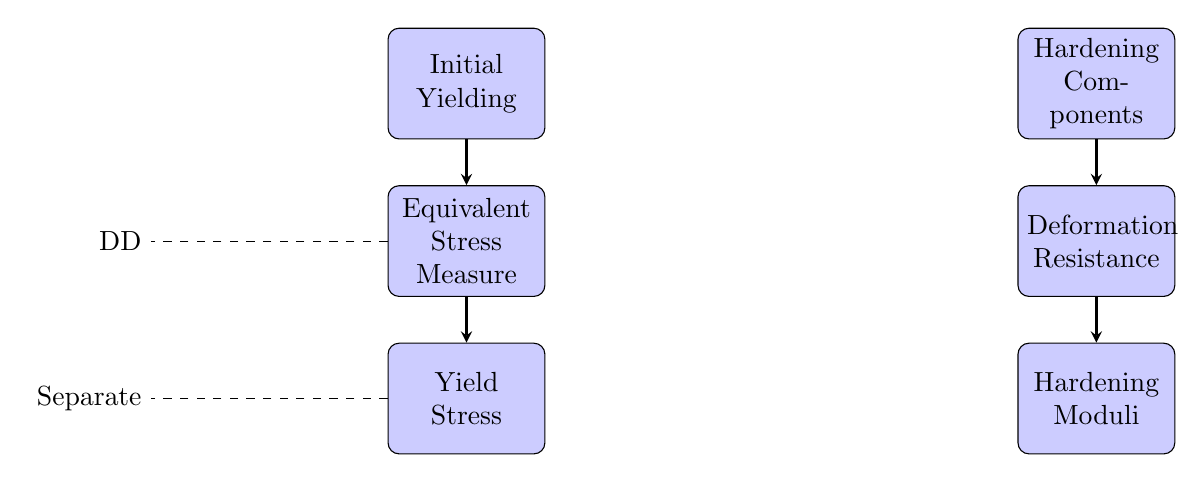
\begin{tikzpicture}[node distance=2cm]

    % Nodes for Initial Yielding
    \node (initial_yielding) [block] {Initial Yielding};
    \node (equiv_stress_measure) [block, below of=initial_yielding] {Equivalent Stress Measure};
    \node (yield_stress) [block, below of=equiv_stress_measure] {Yield Stress};

    % Nodes for Hardening Components
    \node (hardening_components) [block, right of=initial_yielding, xshift=6cm] {Hardening Components};
    \node (deformation_resistance) [block, below of=hardening_components] {Deformation Resistance};
    \node (hardening_moduli) [block, below of=deformation_resistance] {Hardening Moduli};

    % Arrows between nodes
    \draw [arrow] (initial_yielding) -- (equiv_stress_measure);
    \draw [arrow] (equiv_stress_measure) -- (yield_stress);
    \draw [arrow] (hardening_components) -- (deformation_resistance);
    \draw [arrow] (deformation_resistance) -- (hardening_moduli);

    % Lines to indicate modular structure
    \draw[dashed] (equiv_stress_measure.west) -- ++(-3,0) node[left] {DD};
    \draw[dashed] (yield_stress.west) -- ++(-3,0) node[left] {Separate};

\end{tikzpicture}

\end{document}